\usepackage{fontspec}
\usepackage{titlesec}
\usepackage{fancyhdr}
\usepackage{graphicx}
\usepackage{paracol}
\usepackage{anyfontsize}
\usepackage{wrapfig}
\usepackage{tikz}
\usepackage{pythontex}
\usepackage{booktabs}
\usepackage{siunitx}
\usepackage[margin=1cm, top=150pt, headheight=100pt, bottom=2cm]{geometry}
\usepackage[french]{babel}
\selectlanguage{french}
\usepackage{emoji}
\usepackage{braket}

\providefontfamily\Helvetica{Helvetica.ttc}
\providefontfamily\Alice{alice.regular.ttf}
\providefontfamily\Alegreya{alegreya.regular.ttf}
%\providefontfamily\emojiFont{NotoColorEmoji.ttf}
%\providefontfamily\emojiFont{NotoEmoji.ttf}
%\providefontfamily\emojiFont{EmojiOneBW.otf}
%\providefontfamily\emojiFont{EmojiOneColor.otf}
%\providefontfamily\emojiFont{Apple Emoji Color}
%\providefontfamily\emojiFont{Symbola.ttf}
\setemojifont{Apple Color Emoji}

%\setmainfont{Helvetica}
\setlength{\columnsep}{1cm}

\titleformat*{\section}{\Alegreya\Huge}

\fancyhf{}
\fancyfoot[C]{\today}
\fancyhead[L]{
\includegraphics[height=100pt]{logo2.png}}
\fancyhead[R]{\Alice\fontsize{48pt}{52pt}\selectfont Café la Planck}

% Images d'icônes pour certains des avertissements
% Les autres sont des émojis.
\newcommand\moutarde{
\includegraphics[height=12pt]{moutarde.png}}
\newcommand\sesame{
\includegraphics[height=12pt]{sesame.png}}
\newcommand\soja{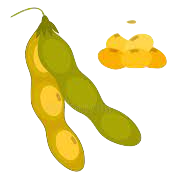
\includegraphics[height=12pt]{soja.png}}
\newcommand\sulfites{
\includegraphics[height=12pt]{sulfites.png}}

\sisetup{table-auto-round, table-format = 1.2, table-alignment-mode = marker, locale=FR, table-column-width=2cm}